\documentclass{article}
% \usepackage{times}
\usepackage{mathptmx}
\usepackage[T1]{fontenc}
\usepackage[latin9]{inputenc}
\usepackage{calc}
\usepackage{units}
\usepackage{amsmath}
\usepackage{amssymb}
\usepackage{graphicx}
\usepackage{subdepth}
\usepackage{cite}
\usepackage{url}
\usepackage{notoccite}
\usepackage{nag}
\title{Newtonian approximation in Causal Dynamical Triangulations}
\author{Adam Getchell}
\date{}
\begin{document}
\maketitle
\tableofcontents

\section{Motivation}

\subsection{Newton's Law of Gravitation from General Relativity}

Starting from the most general cylindrically symmetric (Weyl) metric \cite{synge_relativity}:

\begin{equation}
ds^{2}=e^{2\lambda}dt^{2}-e^{2\left(\nu-\lambda\right)}\left(dr^{2}+dz^{2}\right)-r^{2}e^{-2\lambda}d\phi^{2}\label{eq:weyl-metric}
\end{equation}

\begin{equation}
g_{\mu\nu}=\left(\begin{array}{cccc}
e^{2\lambda}dt^{2} & 0 & 0 & 0\\
0 & -e^{2\left(\nu-\lambda\right)}dr^{2} & 0 & 0\\
0 & 0 & -e^{2\left(\nu-\lambda\right)}dz^{2} & 0\\
0 & 0 & 0 & -\frac{r^{2}}{e^{2\lambda}}d\phi^{2}
\end{array}\right)\label{eq:general-axisymmetric-static-matrix-metric}
\end{equation}

The definition of the Christoffel connection is: \cite{carroll2003spacetime} 
\begin{equation}
\Gamma_{\mu\nu}^{\lambda}=\frac{1}{2}g^{\lambda\sigma}\left(\partial_{\mu}g_{\nu\sigma}+\partial_{\nu}g_{\sigma\mu}-\partial_{\sigma}g_{\mu\nu}\right)
\end{equation}

The non-zero Christoffel connections are:
\begin{equation}
\begin{array}{l}
\Gamma^{t}_{tr}=\partial_{r}\lambda\\
\Gamma^{t}_{tz}=\partial_{z}\lambda\\
\Gamma^{r}_{tt}=e^{4\lambda-2\nu}\partial_{r}\lambda\\
\Gamma^{r}_{rr}=\partial_{r}\nu-\partial_{r}\lambda\\
\Gamma^{r}_{rz}=\partial_{z}\nu-\partial_{z}\lambda\\
\Gamma^{r}_{zz}=\partial_{z}\lambda-\partial_{z}\nu\\
\Gamma^{r}_{\phi\phi}=re^{-2\nu}\left(r\partial_{r}\lambda-1\right)\\
\Gamma^{z}_{tt}=e^{4\lambda-2\nu}\partial_{z}\lambda\\
\Gamma^{z}_{rr}=\partial_{z}\lambda-\partial_{z}\nu\\
\Gamma^{z}_{rz}=\partial_{r}\nu-\partial_{r}\lambda\\ 
\Gamma^{z}_{zz}=\partial_{r}\nu-\partial_{r}\lambda\\
\Gamma^{z}_{\phi\phi}=r^{2}e^{-2\nu}\partial_{z}\lambda\\
\Gamma^{\phi}_{r\phi}=\frac{1}{r}-\partial_{r}\lambda\\
\Gamma^{\phi}_{z\phi}=-\partial_{z}\lambda\\
\end{array}
\end{equation}

The components of the Riemann tensor are given by:
\begin{equation}
R_{\sigma\mu\nu}^{\rho}=\partial_{\mu}\Gamma_{\nu\sigma}^{\rho}-\partial_{\nu}\Gamma_{\mu\sigma}^{\rho}+\Gamma_{\mu\lambda}^{\rho}\Gamma_{\nu\sigma}^{\lambda}-\Gamma_{\nu\lambda}^{\rho}\Gamma_{\mu\sigma}^{\lambda}
\end{equation}

Using the properties of the Riemann tensor:
\begin{equation}
\begin{array}{l}
R_{\rho\sigma\mu\nu}=-R_{\rho\sigma\nu\mu}\\
R_{\rho\sigma\mu\nu}=-R_{\sigma\rho\mu\nu}\\
R_{\rho\sigma\mu\nu}=R_{\mu\nu\rho\sigma}\\
R_{\rho[\sigma\mu\nu]}=0\\
\end{array}
\end{equation}

The non-zero components of the Riemann tensor are:
\begin{equation}
\begin{array}{l}
R^{t}_{rtr}=-\partial^{2}_{r}\lambda+\left(\partial_{z}\lambda\right)^{2}-2\left(\partial_{r}\lambda\right)^{2}+\partial_{r}\lambda\partial_{r}\nu-\partial_{z}\lambda\partial_{z}\nu\\
R^{t}_{rtz}=-\partial_{r}\partial_{z}\lambda-3\partial_{r}\lambda\partial_{z}\lambda+\partial_{r}\lambda\partial_{z}\nu+\partial_{r}\nu\partial_{z}\lambda\\
R^{t}_{ztz}=-\partial^{2}_{z}\lambda-2\left(\partial_{z}\lambda\right)^{2}+\left(\partial_{r}\lambda\right)^{2}-\partial_{r}\lambda\partial_{r}\nu+\partial_{z}\lambda\partial_{z}\nu\\
R^{t}_{\phi t\phi}=re^{-2\nu}\left(r\left(\partial_{r}\lambda\right)^{2}-\partial_{r}\lambda+r\left(\partial_{z}\lambda\right)^{2}\right)\\
R^{r}_{zrz}=\partial^{2}_{r}\lambda-\partial^{2}_{r}\nu+\partial^{2}_{z}\lambda-\partial^{2}_{z}\nu\\
R^{z}_{\phi z\phi}=re^{-2\nu}\left(r\partial^{2}_{z}\lambda-r\partial_{z}\lambda\partial_{z}\nu+r\partial_{r}\lambda\partial_{r}\nu-r\left(\partial_{r}\lambda\right)^{2}+\partial_{r}\lambda-\partial_{r}\nu\right)\\
R^{z}_{\phi\phi r}=re^{-2\nu}\left(-r\partial_{r}\partial_{z}\lambda+r\partial_{r}\nu\partial_{z}\lambda-r\partial_{r}\lambda\partial_{z}\lambda+r\partial_{r}\lambda\partial_{z}\nu-\partial_{z}\nu\right)\\
R^{\phi}_{r\phi r}=\partial^{2}_{r}\lambda+\frac{1}{r}\partial_{r}\nu-\partial_{r}\lambda\partial_{r}\nu-\left(\partial_{z}\lambda\right)^{2}+\partial_{z}\lambda\partial_{z}\nu+\frac{1}{r}\partial_{r}\lambda\\
\end{array}
\end{equation}

The Ricci tensor is given by:
\begin{equation}
R_{\mu\nu}=R_{\mu\lambda\nu}^{\lambda}
\end{equation}

The non-zero components of the Ricci tensor are:
\begin{equation}
\begin{array}{l}
R_{tt}=\frac{e^{4\lambda-2\nu}}{r}\left(r\partial^{2}_{r}\lambda+r\partial^{2}_{z}\lambda+\partial_{r}\lambda\right)\\
R_{rr}=\partial^{2}_{r}\lambda-\partial^{2}_{r}\nu+\partial^{2}_{z}\lambda-\partial^{2}_{z}\nu-2\left(\partial_{r}\lambda\right)^{2}+\frac{1}{r}\partial_{r}\lambda+\frac{1}{r}\partial_{r}\nu\\
R_{rz}=\frac{1}{r}\partial_{z}\nu-2\partial_{r}\lambda\partial_{z}\lambda\\
R_{zz}=\partial^{2}_{r}\lambda-\partial^{2}_{r}\nu+\partial^{2}_{z}\lambda-\partial^{2}_{z}\nu-2\left(\partial_{z}\lambda\right)^{2}+\frac{1}{r}\partial_{r}\lambda-\frac{1}{r}\partial_{r}\nu\\
R_{\phi\phi}=re^{-2\nu}\left(r\partial^{2}_{r}\lambda+r\partial^{2}_{z}\lambda+\partial_{r}\lambda\right)
\end{array}\label{eq:ricci-tensor-components}
\end{equation}

Einstein's equation in a vacuum is:
\begin{equation}
R_{\mu\nu}=0\label{eq:vacuum-solutions}
\end{equation}

Applying this complete set of relations to Equation (\ref{eq:ricci-tensor-components}) gives the following:
\begin{equation}
\partial^{2}_{r}\lambda+\frac{1}{r}\partial_{r}\lambda+\partial^{2}_{z}\lambda=0\label{eq:laplace}
\end{equation}
\begin{equation}
\partial_{r}\nu=r\left(\partial^{2}_{r}\nu+\partial^{2}_{z}\nu+2\left(\partial_{r}\lambda\right)^{2}\right)\label{eq:R_rr=0}
\end{equation}
\begin{equation}
\partial_{z}\nu=2r\partial_{r}\lambda\partial_{z}\lambda\label{eq:nu_z}
\end{equation}
\begin{equation}
\partial^{2}_{r}\nu+\partial^{2}_{z}\nu+\left(\partial_{r}\lambda\right)^{2}+\left(\partial_{z}\lambda\right)^{2}=0\label{eq:R_phiphi=0}
\end{equation}

Equation (\ref{eq:laplace}) is the two-dimensional Laplace equation in cylindrical coordinates, for which the known general solutions are:
\begin{equation}
\lambda (r,z)=\sum^{\infty}_{n=0}[A_{n}J_{n}\left(kr\right)+B_{n}Y_{n}\left(kr\right)][C_{n}\sinh(kz)+D_{n}\cosh(kz)]\label{eq:laplace_sol}
\end{equation}



Plugging Equation (\ref{eq:R_phiphi=0}) into Equation (\ref{eq:R_rr=0}) gives:
\begin{equation}
\partial_{r}\nu=r\left(\left(\partial_{r}\lambda\right)^{2}-\left(\partial_{z}\lambda\right)^{2}\right)\label{eq:nu_r}
\end{equation}

Using Equations (\ref{eq:nu_z}), (\ref{eq:laplace_sol}) and (\ref{eq:nu_r}) we find solutions for $\nu$ given by:
\begin{equation}
\nu=\int r[\left(\left(\partial_{r}\lambda\right)^{2}-\left(\partial_{z}\lambda\right)^{2}\right)dr+\left(2\partial_{r}\lambda\partial_{z}\lambda\right)dz]\label{eq:nu}
\end{equation}


In principle, we have solutions for axially symmetric static vacuum spacetimes. We now wish to add matter. If the object is also axially symmetric and static, then we can consider solutions in the form of an external metric $\emph{E}$ and an internal metric $\emph{I}$, where $\emph{E}$ is given by Equations (\ref{eq:weyl-metric}), (\ref{eq:laplace_sol}), and (\ref{eq:nu}).

The solution of Laplace's equation for a point particle of mass $m$ at $z=z_{0}$ is well known \cite{letelier1997superposition}:

\begin{equation}
\lambda (r,z)=-\frac{m}{\sqrt{r^{2}+\left(z-z_{0}\right)^{2}}}\label{eq:1-m}
\end{equation}

Likewise, we can easily verify for a single particle that the solution for $\nu$ from Equations (\ref{eq:nu}) and (\ref{eq:1-m}) is (setting integration constants equal to zero):
\begin{equation}
\nu (r,z)=-\frac{m^{2}r^{2}}{\left(r^{2}+\left(z-z_{0}\right)^{2}\right)^{2}}
\end{equation}

However, before we can consider this to be a complete solution we must consider elementary flatness. This condition requires that, for any infinitesimal spacelike circle, the ratio of circumference to radius is 2$\pi$. The most likely place to run into issues is along the z-axis, for which $r=0$. Looking back at Equation (\ref{eq:weyl-metric}) we see that the necessary condition is:
\begin{equation}
\lim_{r\rightarrow 0}\nu=0\label{eq:elem-flat}
\end{equation}

Consider the following diagram\footnote{Adapted from Synge} :

\begin{center}
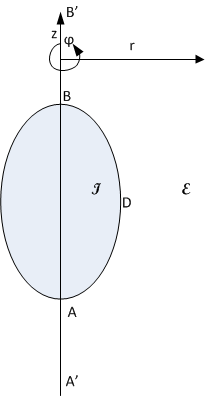
\includegraphics[scale=.75]{Figure1.png}
\end{center}

Equation (\ref{eq:nu}) includes a constant, which we can set by choosing that $\nu=0$ at \emph{A}. So, $\nu=0$ along the z-axis from \emph{A'} to \emph{A}. The same applies from \emph{B} to \emph{B'}. Then our path \emph{ADB} may be deformed into an infinite semicircle.

Now consider two bodies, as in the following diagram:

\begin{center}
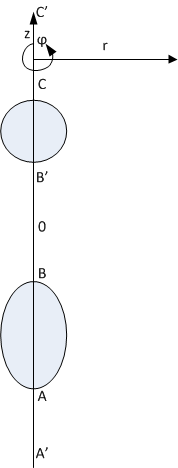
\includegraphics[scale=.75]{Figure2.png}
\end{center}

Since solutions to Laplace's equation are linear, we have:

\begin{equation}
\lambda (r,z)=-\frac{m_{1}}{R_{1}}-\frac{m_{2}}{R_{2}}\label{eq:2-m}
\end{equation}

Plugging this into Equation (\ref{eq:nu}) yields:

\begin{equation}
\nu (r,z)=-\frac{m_{1}^{2}r^{2}}{R_{1}^{4}}-\frac{m_{2}^{2}r^{2}}{R_{2}^{4}}+\frac{4m_{1}m_{2}}{\left(z_{1}-z_{2}\right)^{2}}\frac{r^{2}+\left(z-z_{1}\right)\left(z-z_{2}\right)}{R_{1}R_{2}}
\end{equation}

\begin{equation}
R_{i}=\sqrt{r^{2}+\left(z-z_{i}\right)^{2}}
\end{equation}

In this case, we expect $\nu=0$ along \emph{A'A} and \emph{C'C} as before. But there is no $\emph{a priori}$ reason to think that $\nu=0$ along \emph{B'B}.
This means that our vacuum solution fails along the z-axis. Therefore, there must be a strut of matter, i.e. a metric \emph{I} such that $R_{\mu\nu}\neq 0$, along the z-axis \emph{B'B} separating the two objects. This corresponds with the expectation that two masses will attract each other and not remain at rest.

Indeed, if we apply the condition that $r=0$ we get:

\begin{equation}
\nu (0,z)=\frac{4m_{1}m_{2}}{\left(z_{1}-z_{2}\right)^{2}}
\end{equation}

Which means that in order for Equation (\ref{eq:elem-flat}) to hold, our strut must have:

\begin{equation}
\nu=-\frac{4m_{1}m_{2}}{\left(z_{1}-z_{2}\right)^{2}}
\end{equation}

To get the force on the strut, we can integrate the z-component of the stress-energy tensor over the area:

\begin{equation}
F_{z}=\int T_{zz}d\sigma
\end{equation}

We can get the stress-energy tensor from Einstein's equation:

\begin{equation}
G_{\mu\nu}\equiv R_{\mu\nu}-\frac{1}{2}Rg_{\mu\nu}=8\pi GT_{\mu\nu}
\end{equation}

We have all of the relevant components, except the Ricci scalar:

\begin{equation}
R=R_{\mu}^{\mu}=g^{\mu\nu}R_{\mu\nu}
\end{equation}

Which is:

\begin{equation}
R=2e^{2\left(\lambda-\nu\right)}\left(\partial^{2}_{r}\nu+\partial^{2}_{z}\nu-\partial^{2}_{r}\lambda-\partial^{2}_{z}\lambda+\left(\partial_{r}\lambda\right)^{2}+\left(\partial_{z}\lambda\right)^{2}-\frac{1}{r}\partial_{r}\lambda\right)\label{eq:R}
\end{equation}

Recall that earlier we asserted in Equation (\ref{eq:vacuum-solutions}) that we had a vacuum solution. In order for this to be true, our Ricci scalar better be equal to zero, since a vacuum solution actually corresponds to:

\begin{equation}
G_{\mu\nu}=0
\end{equation}

Using Equations (\ref{eq:laplace}) and (\ref{eq:R_phiphi=0}) and plugging them into Equation (\ref{eq:R}) we see that this is indeed the case.

Continuing, we get:

\begin{equation}
G_{zz}=\left(\partial_{r}\lambda\right)^{2}-\left(\partial_{z}\lambda\right)^{2}-\frac{1}{r}\partial_{r}\nu
\end{equation}

Thus:

\begin{equation}
T_{zz}=\frac{1}{8\pi G}(stuff hopefully \nu)
\end{equation}
\bibliographystyle{ieeetr}
\bibliography{cdt-newtonian-limit-biblio}


\end{document}
